\chapter{Numerical Computations for the Five Point Function}
The one loop integrals play an important role in calculating radiative corrections in particle physics since they are manageable for fast MC event generator execution for arbitrary masses and kinematics for high energy scattering process. It has been demonstrated that $n$-point functions at one-loop level can be reduced to scalar one loop functions \cite{Denner, PV}. Considering representations of the scalar four-point function for arbitrary masses and momenta relevant to most high energy collider applications have been given and they fit MC implementation well, it is natural to attempt expressing higher point-function ($n\ge5$) in terms of the 1, 2, 3 and 4-point functions. When the problem becomes reducing higher-point functions into expressions in terms of the 1,2,3 and 4-point functions, we are most concerned about the numerical stability. To solve this problem,  B. F. L. Ward presented an approach to evaluate higher point loop integrals using Chinese magic in the virtual loop integration variable \cite{MagicSpinor}, which is called "magic spinor product methods in loop integrals". Based on this method, we developed a program to compute the general five-point function numerically. In this Chapter, we first introduce the physics content of "magic spinor product methods in loop integrals" and then we compare our results with those from LoopTools \cite{LT}, which is a package for computation of one-loop integrals based on the FF package by G. J. van. Oldenborgh\cite{vOV90}. By comparison, it shows the result from our program is accurate and numerically stable.





\section{Magic Spinor Product Approach in Loop Integrals}



Here we use the conventions of Refs. \cite{GPS,JWZ2001prd} which are derived from Refs. \cite{ChnMag,KS}. The five-point function which we analyze is shown in diagram (c). It has many applications in collider precision physics. For example, together with diagrams (a) and (b) it generates a gauge invariant contribution to the ISR for $e^+e^-\to f\bar{f}+\gamma$, $f\neq e$. We focus on the application of Chinese magic in the loop integral in Fig.(c) to illustrate the possible simplifications here.

\begin{center}
	\begin{axopicture}(520,210)
		\Photon(50,170)(130,170){3}{7}
		\Photon(50,90)(130,90){3}{7}
		\Line(50,90)(50,170) 
		\Line(130,90)(130,170)
		\Line[arrow](5,215)(27.5,192.5)\Line[arrow](27.5,192.5)(50,170)\Text(0,210){$p_1$}
		\Photon(27.5,192.5)(57.5,222.5){2}{5}
		\Line[arrow](175,215)(130,170)\Text(160,210){$p_4$}
		\Line[arrow](5,45)(50,90)  \Text(0,50){$p_2$} 
		\Line[arrow](175,45)(130,90) \Text(160,50){$p_3$}
		\Text(67.5,220){$k$}
		\Text(90,180){$q$}
		\Text(90,20){(a)}
		
		\Photon(260,170)(340,170){3}{7}
		\Photon(260,90)(340,90){3}{7}
		\Line(260,90)(260,170)  
		\Line(340,90)(340,170)
		\Line[arrow](215,215)(260,170)
		\Line[arrow](385,215)(340,170)
		\Line[arrow](215,45)(237.5,67.5)\Line[arrow](237.5,67.5)(260,90)
		\Line[arrow](385,45)(340,90)
		\Text(210,50){$p_2$} 
		\Text(210,210){$p_1$}
		\Text(370,210){$p_4$}
		\Text(370,50){$p_3$}
		\Photon(237.5,67.5)(267.5,37.5){2}{5}
		\Text(270,45){$k$}
		\Text(300,180){$q$}
		\Text(300,20){(b)}
	\end{axopicture}
\end{center}

\begin{center}
	\begin{axopicture}(260,210)
		
		\Photon(50,170)(130,170){3}{7}
		\Photon(50,90)(130,90){3}{7}
		\Line(50,90)(50,130)\Line(50,130)(50,170)
		\Photon(5,130)(50,130){2}{5} \Text(0,130){$k$}
		\Line(130,90)(130,170)
		\Line[arrow](5,215)(50,170)\Text(0,210){$p_1$}
		
		\Line[arrow](175,215)(130,170)\Text(160,210){$p_4$}
		\Line[arrow](5,45)(50,90)  \Text(0,50){$p_2$} 
		\Line[arrow](175,45)(130,90) \Text(160,50){$p_3$}
		\Text(90,180){$q$}
		\Text(90,20){(c)}
		
	\end{axopicture}
	\\{\sl ISR five-point function contributions with fermion and vector boson mases $m_f$, $m_B$, $f=1,2$, $B=V_1,V_2$ and with momenta $p_i$, $k$ with $Q\equiv p_1+p_2$.$p_1$ is the incoming fermion momentum, $p_2$ is the incoming antifermion momentum and $k$ is the real photon momentum.}
\end{center}



 Applying the Feynman rules, we have
\begin{eqnarray}
&&M^{(1c)}_{\lambda_1\lambda_2\lambda'_1\lambda'_2\lambda_\gamma}=(2\pi)^4\delta(p_1+p_2-p'_1-p'_2-k)\mathcal{C}\nonumber\\
&&\times\int\frac{d^4q}{(2\pi)^4}\frac{\bar{v}_{\lambda_2}\gamma^\beta(\slashed q+\slashed p_1-\slashed k+m_1)\slashed \epsilon_{\lambda_\gamma}^\ast(\slashed q+\slashed p_1+m_1)\gamma^\alpha u_{\lambda 1}}{[(q+p_1-k)^2-m_1^2+i\epsilon][(q+p_1)^2-m_1^2+i\epsilon]}\nonumber\\
&&\frac{\bar{u}'_{\lambda'_1}\gamma_\alpha(\slashed q+\slashed p'_1+m_2)\gamma_\beta v'_{\lambda'_2}}{[(q+p_1+p_2-k)^2-M_{V_2}^2+i\epsilon][(q+p_{1}^{'2})^2-m_2^2+i\epsilon](q^2-M_{V_1}^2+i\epsilon)}\nonumber\\
&&+\cdots,
\end{eqnarray}
where we define massless limit coupling factor
\begin{eqnarray}
\mathcal{C}&=&\mathcal{C}({\lambda_i},{\lambda'_j})\nonumber\\
&=&Q_1eG^2G'^2(v'_1+a'_1\lambda_2)(v_1-a_1\lambda_1)(v'_2+a'_2\lambda_2)(v_2+a_2\lambda'_1)
\end{eqnarray}	
with the couplings $Q_1e$, $G$, and $G'$ for the $\gamma$, $V_1$ and $V_2$ respectively. In order to obtain the loop integral in terms of Chinese magic, we take the following kinematics
\begin{align}
p_1&=(E,p\hat{z})\nonumber\\
p_2&=(E,-p\hat{z})\nonumber\\
-p_4&=(E',p'(\cos\theta'_1\hat{z}+\sin\theta'_1\hat{x}))\equiv p'_1\nonumber\\
k&=(k_0,k(\cos\theta_\gamma\hat{z}+\sin\theta_\gamma(\cos\phi_\gamma\hat{x}+\sin\phi_\gamma\hat{y})))\nonumber\\
p_1+p_2&=-p_4-p_3+k=(\sqrt{s},\vec{0})\nonumber\\
-p_3&\equiv p'_2,
\end{align}
with $k^0=k$, $\sqrt{s}=2E$. Besides, we introduce the alternative notations $p'_1=-p_4$, $p'_2=-p_3$. Now we introduce the two sets of magic polarization vectors asscociated to the two incoming lines
\begin{eqnarray}
(\epsilon^\mu_\sigma(\beta))^\ast&=&\frac{\bar{u}_\sigma(k)\gamma^\mu u_\sigma(\beta)}{\sqrt{2}\bar{u}_{-\sigma}u_\sigma(\beta)},\nonumber\\
(\epsilon^\mu_\sigma(\zeta))^\ast&=&\frac{\bar{u}_\sigma(k)\gamma^\mu u_\sigma(\zeta)}{\sqrt{2}\bar{u}_{-\sigma}u_\sigma(\zeta)},
\end{eqnarray}
with $\beta^2=0$ and $\zeta^2=0$. We choose the basis of the four-dimensional momentum space as follows:
\begin{align}
\ell_1&=(E,E\hat{z})\nonumber\\
\ell_2&=(E,-E\hat{z})\nonumber\\
\ell_3&=E\frac{\braket{\ell_2+|\gamma^\mu|\ell_1+}}{\sqrt{2}\braket{\ell_2-|\ell_1+}}=-\frac{E}{\sqrt{2}}(\hat{x}+i\hat{y})\nonumber\\
\ell_4&=E\frac{\braket{\ell_2-|\gamma^\mu|\ell_1-}}{\sqrt{2}\braket{\ell_2+|\ell_1-}}=\frac{E}{\sqrt{2}}(\hat{x}-i\hat{y})
\end{align}
where we use the Dirac notations in Refs. \cite{CALKUL,KS,MagicSpinor}. Note that all four of the basis four-vector are lightlike so that they can attend in Chinese magic. 

We define the loop momentum as

\begin{equation}
q=\alpha_i\ell_i
\end{equation}
with summation over repeated indices. The coefficient $\alpha_i$'s are dertermined as
\begin{align}
\alpha_1&=\frac{q\ell_2}{2E^2}=\frac{1}{s}(D_3-D_2-s+2p_2k+M^2_{V_2}),\nonumber\\
\alpha_2&=\frac{q\ell_1}{2E^2}=\frac{1}{s}(D_1-D_0-M^2_{V_1}),\nonumber\\
\alpha_3&=\frac{q\ell_4}{E^2}=-\frac{q\ell_3^\ast}{E^2}=-\alpha_4^\ast,\nonumber\\
\alpha_4&=-\frac{i}{\sqrt{2s}}[c_jD_j+c_5M_{V_1}^2+c_6(M^2_{V_2}+2p_2k-s)+c_7(2kp_1)],
\end{align}
where we define the denominators as
\begin{align}
D_0&=q^2-M^2_{V_1}+i\epsilon\nonumber\\
D_1&=(q+p_1)^2-m_1^2+i\epsilon\nonumber\\
D_2&={q+p_1-k}^2-m^2_{1}+i\epsilon\nonumber\\
D_3&={q+p_1+p_2-k}^2-M^2_{V_2}+i\epsilon\nonumber\\
D_4&=(q-p_4)^2-m^2_2+i\epsilon
\end{align}
such that the expansion coefficents $\{c_j\}$ are
\begin{align}
c_0&=\csc\phi_\gamma\left(\frac{\csc\theta'_1e^{i\phi_\gamma}}{\beta'_1E'_1}-\frac{\csc\theta'_1e^{i\phi_\gamma}}{\beta'_1\sqrt{s}}+\frac{\csc\theta_\gamma}{\sqrt{s}}-\frac{\cot\theta'_1e^{i\phi_\gamma}-\cot\theta_\gamma}{\beta_1\sqrt{s}} \right),\nonumber\\
c_1&=\csc\phi_\gamma\left(\frac{\csc\theta'_1e^{i\phi_\gamma}}{\beta'_1\sqrt{s}}-\frac{\csc\theta'_1}{\sqrt{s}}+\frac{\cot\theta'_1e^{i\phi_\gamma}-\cot\theta_\gamma}{\beta_1\sqrt{s}}+\frac{\csc\theta_\gamma}{k^0} \right),\nonumber\\
c_2&=\csc\phi_\gamma\left(\frac{-\csc\theta'_1e^{i\phi_\gamma}}{\beta'_1\sqrt{s}}+\frac{\csc\theta_\gamma}{\sqrt{s}}+\frac{\cot\theta'_1e^{i\phi_\gamma}-\cot\theta_\gamma}{\beta_1\sqrt{s}}-\frac{\csc\theta_\gamma}{k^0} \right),\nonumber\\
c_3&=\csc\phi_\gamma\left(\frac{\csc\theta'_1e^{i\phi_\gamma}}{\beta'_1\sqrt{s}}-\frac{\csc\theta_\gamma}{\sqrt{s}}-\frac{\cot\theta'_1e^{i\phi_\gamma}-\cot\theta_\gamma}{\beta_1\sqrt{s}}\right),\nonumber\\
c_4&=-\csc\phi_\gamma\frac{\csc\theta'_1e^{i\phi_\gamma}}{\beta'_1E'_1},\nonumber\\
c_5&=\csc\phi_\gamma\left(\frac{\csc\theta'_1e^{i\phi_\gamma}}{\beta'_1E'_1}-\frac{\csc\theta'_1e^{i\phi_\gamma}}{\beta'_1\sqrt{s}}+\frac{\csc\theta_\gamma}{\sqrt{s}}-\frac{\cot\theta'_1e^{i\phi_\gamma}-\cot\theta_\gamma}{\beta_1\sqrt{s}} \right),\nonumber\\
c_6&=\csc\phi_\gamma\left(\frac{\csc\theta'_1e^{i\phi_\gamma}}{\beta'_1\sqrt{s}}-\frac{\csc\theta_\gamma}{\sqrt{s}}-\frac{\cot\theta'_1e^{i\phi_\gamma}-\cot\theta_\gamma}{\beta_1\sqrt{s}}\right),\nonumber\\
c_7&=-\csc\phi_\gamma\frac{\csc\theta_\gamma}{k^0},
\end{align}
with $\beta=\frac{p}{E}$ and $\beta'_1=\frac{p'}{E'}$. Therefore the $\{c_j\}$ are determined by the kinematics that we choose. Note that the Chinese magic now carries over to the loop variable via the identity
\begin{align}
\slashed q&=\alpha_j\slashed \ell_j\nonumber\\
&=\sum_{j=1}^{2}\alpha_j(\ket{\ell_j+}\bra{\ell_j+}+\ket{\ell_j-}\bra{\ell_j-})+\alpha_3\frac{\sqrt{2}E}{\braket{p_2-|p_1+}}(\ket{\ell_2-}\bra{\ell_1-}+\ket{\ell_1-}\bra{\ell_2+})\nonumber\\
&+\alpha_4\frac{\sqrt{2}E}{\braket{p_2+|p_1-}}(\ket{\ell_2+}\bra{\ell_1+}+\ket{\ell_1-}\bra{\ell_2-})\nonumber\\
&\equiv\sum_{j=1}^{2}\alpha_j(\ket{p_j+}\bra{p_j+}+\ket{p_j-}\bra{p_j-})+\alpha_3\frac{\sqrt{2}E}{\braket{p_2-|p_1+}}(\ket{p_2-}\bra{p_1-}+\ket{p_1-}\bra{p_2+})\nonumber\\
&+\alpha_4\frac{\sqrt{2}E}{\braket{p_2+|p_1-}}(\ket{p_2+}\bra{p_1+}+\ket{p_1-}\bra{p_2-})\nonumber\\
&\equiv\sum_{j=1}^{2}\alpha_j(\ket{p_j+}\bra{p_j+}+\ket{p_j-}\bra{p_j-})+\widetilde{\alpha}_3(\ket{p_2-}\bra{p_1-}+\ket{p_1-}\bra{p_2+})\nonumber\\
&+\widetilde{\alpha}_4(\ket{p_2+}\bra{p_1+}+\ket{p_1-}\bra{p_2-}),
\end{align}
where we let $\ell_1\equiv p_1$, $\ell_2\equiv p_2$ since for the numeratior algebra we work in the massless limit. And we define as well
\begin{align}
\widetilde{\alpha}_3&\equiv\alpha_3\frac{\sqrt{2}E}{\braket{p_2-|p_1+}}=-\frac{\alpha_3}{\sqrt{2}},\nonumber\\
\widetilde{\alpha}_4&\equiv\alpha_4\frac{\sqrt{2}E}{\braket{p_2+|p_1-}}=-\frac{\alpha_4}{\sqrt{2}}.
\end{align}


Next, we introduce the representation (4.10) into the numerator, $N$, of the integrand in eq (4.1). Then we have the reduction
\begin{align}
N&=\frac{4\sqrt{2}}{\braket{k-|p_1+}}\{ (A_1\braket{p_2+|p'_1-}\braket{p'_2-|p_2+}\nonumber\\
& +A_2\braket{p_2+|p'_1-}\braket{p'_2-|p_1+} )\times(A_3\braket{p_2+|p'_1-}\braket{p'_1-|p_1+}\nonumber\\
& +A_4\braket{p_1+|p'_1-}\braket{p'_1-|p_1+} ) \nonumber\\
&+\widetilde{\alpha}_4 (A_1\braket{p_2+|p_1-}\braket{p'_2-|p_2+} +A_2\braket{p_2+|p_1-}\braket{p'_2-|p_1+} )
\nonumber\\
&\times(A_3\braket{p_2+|p'_1-}\braket{p_2-|p_1+}\nonumber\\
& +A_4\braket{p_1+|p'_1-}\braket{p_2-|p_1+} ) \}
\end{align}
from the standard identities
\begin{align}
\slashed \epsilon_{\lambda_\gamma}^\ast&=\frac{\sqrt{2}}{\braket{k-\lambda_\gamma|\ell_1\lambda_\gamma}}[\ket{\ell_1\lambda_\gamma}\bra{k\lambda_\gamma}+\ket{k-\lambda_\gamma}\bra{\ell_1-\lambda_\gamma}],\nonumber\\
\gamma^\rho\braket{\ell_1\lambda|\gamma_\rho|\ell_2\lambda}&=2[\ket{\ell_1-\lambda}\bra{\ell_2-\lambda}+\ket{\ell_2\lambda}\bra{\ell_1\lambda}],\nonumber\\
\slashed\ell_1&=\ket{\ell_1+}\bra{\ell_1+}+\ket{\ell_1-}\bra{\ell_1-},
\end{align}
where we defined
\begin{equation}
\begin{cases}
A_1=\widetilde{\alpha}_4\braket{p_1+|k-}+\alpha_2\braket{p_2+|k-},
\\
A_2=(1+\alpha_1)\braket{p_1+|k-}+\widetilde{\alpha}_3\braket{p_2+|k-},\\
A_3=\alpha_2\braket{p_1-|p_2+},\\
A_4=\widetilde{\alpha}_4\braket{p_1-|p_2+},
\end{cases}
\end{equation}
for the magic choice $\beta=p_1$. Note that the Chinese magic trick has eliminated all but one set of the terms with three factors of the virtual momentum expansion coefficients. Moreover, in the numerator of the propagator before or after the real emission vertex, this trick has annihilated the terms associated with $\slashed p_1\slashed k$ as well as half of the terms in the respective virtual momentum expansion in the former case. Compared to the traditional approach of taking traces on the fermion lines, the Chinese magic trick has a large fraction of the terms on the right-hand side of eq. (4.12). Specifically speaking, We need to compute $2\Re\mathcal{M}_B^\ast\mathcal{M}^{(1c)}$ in the usual method of taking traces of fermion lines, where $\mathcal{M}_B$ is the respective Born amplitude that would interfere with the one-loop amplitude to generate the one-loop correction ot the respective cross section. In the Chinese magic representation, we find that only radiation from the antifermion ($p_2$) incoming line contributes.  
\begin{align}
\mathcal{M}_{B+-+-+}=&(2\pi)^4\delta(p_1+p_2-p'_1-p'_2-k)\nonumber\\
&\times\frac{2\sqrt{2}ieQ_1G_j^2(v'_j-a'_j)(v_j-a_j)\braket{p'_2-|p_1+}}{\braket{k-|p_1+}\braket{k-|p_2+}(s'-M_{V_j}^2+i\epsilon)}\nonumber\\
&\times[\braket{p_1-|p_2+}\braket{p_2+|p'_1-}-\braket{p_1-|k+}\braket{k+|p'_1-}].\nonumber\\
\end{align}
Therefore the calculation for $2\Re\mathcal{M}_B^\ast\mathcal{M}^(1c)$ just involves multiplying $N$ in eq. (4.12) by the complex conjugate of the simple expression and taking twice the real part.

Assume that the traditional approach of taking traces of fermion lines is applied, we need the trace of two sets of terms with 10 Dirac gamma matrices multiplied by a factor with the trace of 6 Dirac gamma matrices. If so, we will have $2\cdot9\cdot7\cdot5\cdot4\times5\cdot4=2520\times20=50400$ terms. Each terms requires Passarino-Veltman (PV) reduction of three, two, and one five-point tensor integrals. By comparison, we can appreciate the great simplification that eq. (4.12) represents. We see that this form of $N$ in eq. (4.12) has efficiently reduced the problem of reduction of the five-point function with three, two, one tensor indices in the PV scheme to the question of a single scalar five-point and lower four, three, and two point functions with the coefficients already explicitly written in terms of the center of mass (CMS) kinematic variables which are important to efficient MC generations. Furthermore, if we introduce the result of $N$ in eq. (4.12) into the integral in eq. (4.1), we have the integrals

\begin{equation}
\int \frac{d^4q}{(2\pi)^4}\frac{D_iD_jD_k;D_iD_j;D_j;1}{D_0D_1D_2D_3D_4},\quad i,j,k=0,\cdots,4
\end{equation}
all of which are determined from the lower point functions when the results for the representation of the scalar five-point function in terms of four-point functions used in Refs. \cite{tHscarlar,WJ,DD,DD1}. Then we obtain an advantage: no calculation of wave functions at complex momenta is required here. Our work results rigorously from Lagrangian quantum field theory and thus it could be used as a cross check on other possible approaches. 


So far we have simplified considerably the computation and have removed the Gram determinant-type factors in the tensor integral redcutions. But our calculation sill depends on the Gram determinant-type denominator factors in the results in Refs. \cite{tHscarlar,WJ,DD,DD1} for the representation of the five-point function in terms of scalar four-point functions. In order to achieve a better numerical stability, we need to replace the representation of the scalar five-point function.
 
Let us begin with the identity
\begin{align}
q^2&=D_0+M_{V_1}^2-i\epsilon=(\alpha_i\ell_i)^2\nonumber\\
&=2\alpha_1\alpha_2\ell_1\ell_2+2\alpha_3\alpha_4\ell_3\ell_4=s\alpha_1\alpha_2+\frac{s}{2}\alpha_3\alpha_4.
\end{align}

Dividing by $D_0\cdots D_4$ and integrating over $d^4q$ we have the following representation of the required scalar five-point function
\begin{align}
&E_0(\bar{p}_1,\bar{p}_2,\bar{p}_3,\bar{p}_4,\bar{m}_0,\bar{m}_1,\bar{m}_2,\bar{m}_3,\bar{m}_4)\nonumber\\
&=\frac{1}{C_{E_0}}\biggl\{-D_0(0)+\frac{1+\beta_1^2}{2s\beta_1^2}\bigg[C_0(13)-C_0(12)-C_0(03)+C_0(02)\nonumber\\
&+(M_{V_2}^2-s+2p_2k) 
\bigg(D_0(1)-D_0(0)\bigg)-M^2_{V_1}\bigg(D_0(3)-D_0(2)\bigg)    \bigg]   \nonumber\\
&-\frac{1-\beta_1^2}{4s\beta_1^2}\bigg[\Delta r_{1,0}\bigg(D_0(1)-D_0(0)\bigg)+2\Delta\bar{p}_{1,0}\bigg( D_{11}(1)\bar{\bar{p}}(1)_1-D_{11}(0)\bar{\bar{p}}(0)_1\nonumber\\&+D_{12}(1)\bar{\bar{p}}(1)_2-D_{12}(0)\bar{\bar{p}}(0)_2+D_{13}(1)\bar{\bar{p}}(1)_3-D_{13}(2)\bar{\bar{p}}(2)_3-D_{0}(3)\bar{\bar{p}}(3)_4\nonumber\\
& +D_{0}(2)\bar{\bar{p}}(2)_4 \bigg) +2(M_{V_2}^2-s+2p_2k)\bigg(D_0(3)-D_0(2)\bigg) \bigg]  \nonumber\\
&-\frac{1}{4}\bigg[\sum_{j=0}^{4}|c_j|^2\bigg(C_0(j,j+1)+\Delta r_{j,j+1}D_0(j)+2\Delta\bar{p}_{j,j+1} (D_{11}(j)\bar{\bar{p}}(j)_1 \nonumber\\
&+D_{12}(j)\bar{\bar{p}}(j)_2+D_{13}(j)\bar{\bar{p}}(j)_3-D_{0}(j)\bar{\bar{p}}(j)_4   ) \bigg)  \nonumber\\
&+2\bigg( \sum_{i>j}^{4}\Re(c_ic^\ast_j)C_0(ij)+\sum_{j=0}^{4}\Re(c_j(c_5^\ast M_{V_1}^2+c_6^\ast(M^2_{V_2}-s+2p_2k)+c_7^\ast(2kp_1))  )\nonumber\\
&D_0(j) \bigg)\bigg]\biggr\}
\end{align}
where
$\bar{p}=p_1$, $\bar{p}_2=p_1-k$, $\bar{p}_3=p_1+p_2-k$, $\bar{p}=p'_1$, $\bar{m_0}-M_{V_1}$, $\bar{m}_1=m_1$, $\bar{m}=m_1$, $\bar{m}_3=M_{V_2}$, $\bar{m}_4=m_2$,
where the coefficient $C_{E_0}$ is 
\begin{align}
C_{E_0}=&M^2_{V_1}-i\epsilon+\frac{1+\beta_1^2}{2\beta_1^2s}M^2_{V_1}(M^2_{V_2}-s+2p_2k)+\frac{1-\beta_1^2}{4\beta_1^2s}(M^4_{V_1} \nonumber\\
&+(M^2_{V_2}-s+2p_2k)^2)+\frac{1}{2}\Re[c_5c_6^\ast M^2_{V_1}(M_{V_2}^2-s+2p_2k)  \nonumber\\
&+c_5c_7^\ast M^2_{V_1}(2kp_1)  +c_6c_7^\ast(M^2_{V_2}-s+2p_2k)(2kp_1)  ]\nonumber\\
&+\frac{1}{4}[|c_5|^2M^4_{V_1}+|c_6|^2(M_{V_2}^2-s+2p_2k)^2+|c_7|^2(2kp_1)^2].
\end{align}
We have used a mixture of notations from \cite{PV,WJ,DD,DD1} such that
\begin{align}
D_j&=(q-\bar{p}_j)^2-\bar{m}^2_j+i\epsilon=q^2+2q\bar{p}_j+\bar{p}^2_j-\bar{m}^2_j+i\epsilon\equiv q^2+2q\bar{p}_j+r_j,\nonumber\\
\Delta_{i,j}&\equiv r_i-r_j,\nonumber\\
\Delta\bar{p}_{i,j}&\equiv\bar{p}_i-\bar{p}_j\nonumber\\
D_0(j)&\equiv\text{four-point scalar function obtained from five-point scalar function}\nonumber\\
&\text{by omitting denominatror} D_j,\nonumber\\
C_0(i,j)&\equiv\text{three-point scalar function obtained from five-point scalar function}\nonumber\\
	&\text{by omitting denominatror} D_i \text{ and } D_j, i\neq j \nonumber\\
\end{align}
where we also use the Passarino-Veltman \cite{PV} notation of the four-point one-tensor integral, $D_\mu(j)$, obtained from the five-point one tensor integral function by omitting the denominator $D_j$, with
$$D_\mu(j)\equiv D_{11}(j)\bar{\bar{p}}(j)_1+D_{12}(j)\bar{\bar{p}}(j)_2+D_{13}(j)\bar{\bar{p}}(j)_3-D_{0}(j)\bar{\bar{p}}(j)_4,
$$
where the four-vectors $\{\bar{\bar{p}}(j)_j\}$ are determined according to Ref. \cite{PV}. Note that $\bar{\bar{p}}(j)_4$ is only nonzero if it is necessary to shift the $q$-integration variable by it to reach the standard form of Passarino-Veltman representation. This expression for $E_0$ have no problem with Gram determinant type denominators.


\begin{align}
\mathcal{M}^(1a)_{+-+-+}&=0,\text{  by Chinese magic trick}\nonumber\\
\mathcal{M}^(1b)_{+-+-+}&=(2\pi)^4\delta (p_1+p_2-p'_1-p'_2-k)\nonumber\\
&\times\frac{4\sqrt{2}\mathcal{C}}{\braket{k-|p_1+}\braket{k-|p_2+}}\int\frac{d^4q}{(2\pi)^4}\frac{N'}{D_0D_1D_3D_4},
\end{align}
where the numerator $N'$ is given by
\begin{align}
N'=&(\braket{p'_2-|p_1+}a_1+\braket{p'_2-|p_2+}b_1)\nonumber\\
&\times(\braket{p_1-|p_2+}\braket{p_2+|p'_1-}-\braket{p_1-|k+}\braket{k+|p'_1-})\nonumber\\
&+(\braket{p'_2-|p_1+}\bar{a}_1+\braket{p'_2-|p_2+}\bar{b}_1)\nonumber\\
&\times[-2p_1(p_2-k)\widetilde{\alpha}_4+\alpha_2\braket{p_1-|k+}\braket{k+|p_2-}]
\end{align}
with
\begin{align}
a_1&=(1+\alpha_1)(2p_1p'_1)+\alpha_3\braket{p_2+|p'_-}\braket{p'_1-|p_1+},\nonumber\\
b_1&=\alpha_2\braket{p_2+|p'_1-}\braket{p'_1-|p_1+}+\widetilde{\alpha}_4(2p_1p'_1),\nonumber\\
\bar{a}_1&=\braket{p_1-|p_2+}[(1+\alpha_1)\braket{p_1+|p'_1-}+\widetilde{\alpha}_3\braket{p_2+|p'_1-}],\nonumber\\
\bar{b}_1&=\braket{p_1-|p_2+}[\alpha_2\braket{p_2+|p'_1-}+\widetilde{\alpha}_4\braket{p_1+|p'_1-}].
\end{align}
As we see this method gives a considerable reduction to the known scalar functions  while computing $2\Re\mathcal{M}_B^\ast\mathcal{M}^{1b}$ compared to the traditional method of tracing over fermion lines.

In sum, we have exhibited that the application of Chinese magic technique in the virtual loop momentum could reduce significantly the volume of algebra required for efficient and stable physical calculations of higher point virtual corrections with the general mass scale. Furthermore, we could construct computer realizations of the method described above for evaluating the five-point function. In the next section, we will exhibit our results and compare them with those from LoopTools.
\newpage
\section{Numerical Results for the Five-Point Function $E_0$}
Based on the magic spinor product method, we have developed a computer program to calculate the five-point function $E_0$. In our program, the LoopTools package is included. The five-point function $E_0$ is calculated with the help of eqs. (4.9), (4.18) and (4.19). Scalar three-point functions $C_0(i,j)$, scalar four-point functions $D_0(j)$ and tensor four-point functions $D_{\mu\nu}(j)$ are calculated by Looptools. To be specific, we choose
\begin{equation*}
\begin{cases}
\sqrt{s}=500\text{ GeV},\\
m_1=m_e=0.510999\times 10^{-3}\text{ GeV},\\
m_2=m_\mu=0.1056583\text{ GeV},\\
M_{V_1}=M_{V_2}=91\text{ GeV},
\end{cases}
\end{equation*}
and the kinematics is determined by eq. (4.3).

\begin{center}
	\begin{axopicture}(210,200)
		\Photon(60,140)(60,60){3}{6}
		\Line(60,140)(100,140)\Line(100,140)(140,140)
		\Photon(140,140)(140,60){3}{6}
		\Line(60,60)(140,60)
		\Line[arrow](15,185)(60,140)
		\Line[arrow](185,185)(140,140)
		\Line[arrow](15,15)(60,60)
		\Line[arrow](185,15)(140,60)
		\Photon(100,140)(100,190){3}{5}
		\Text(10,190){$p_1$}
		\Text(190,190){$p_2$}
		\Text(190,10){$p_3$}
		\Text(10,10){$p_4$}
		\Text(100,200){$k$}
		\Text(80,145){$m_1$}
		\Text(120,145){$m_2$}
		\Text(45,100){$M_{V_1}$}
		\Text(155,100){$M_{V_2}$}
		\Text(100,50){$m_5$}
	\end{axopicture}
\end{center}
then by eq. (4.8) and (4.20), we have the expressions of $D_0(j)$ and $C_0(i,j)$ which give inputs of the corresponding three- and four-point functions in Looptools so that we can compute $D_0(j)$, $C_0(i,j)$ and $D_{\mu\nu}(i,j)$ via Looptools. Besides, we have computed $E_0$ via Looptools directly as a comparision. We choose $(\phi_\gamma,\theta_\gamma,\theta'_1)$ as the variables. The percent Differences of $E_0(\phi_\gamma,\theta_\gamma)$ and $E_0^{looptools}(\phi_\gamma,\theta_\gamma)$ are shown in Figure (4.1)-(4.13).


\begin{figure}
	\begin{center}
		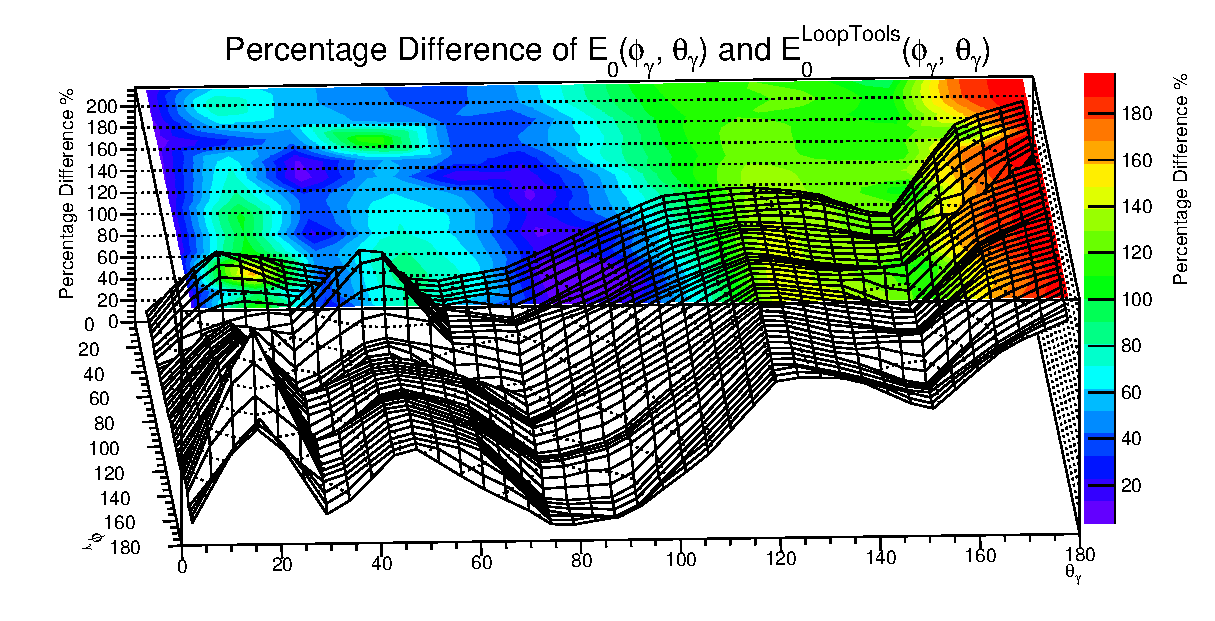
\includegraphics[scale=0.55]{0PD3.eps}
		\caption{ Percentage difference of $E_0(\phi_\gamma,\theta_\gamma)$ and $E_0^{LoopTools}(\phi_\gamma,\theta_\gamma)$ for $\sqrt{s}=500\text{ GeV}$, $M_{V_1}=91\text{ GeV}$, $M_{V_1}=91\text{ GeV}$ and $\theta'_1=0$ }
	\end{center}
\end{figure}

\begin{figure}
	\begin{center}
		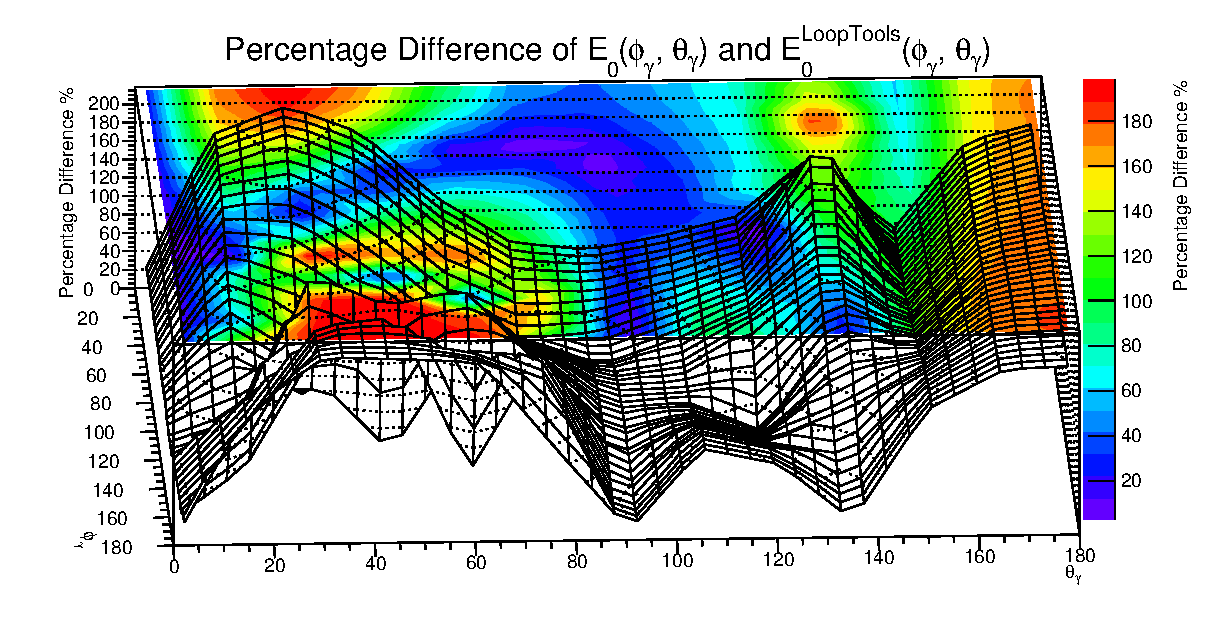
\includegraphics[scale=0.55]{15PD3.eps}
	\caption{ Percentage difference of $E_0(\phi_\gamma,\theta_\gamma)$ and $E_0^{LoopTools}(\phi_\gamma,\theta_\gamma)$ for $\sqrt{s}=500\text{ GeV}$, $M_{V_1}=91\text{ GeV}$, $M_{V_1}=91\text{ GeV}$ and $\theta'_1=15$ }
	\end{center}
\end{figure}

\begin{figure}
	\begin{center}
		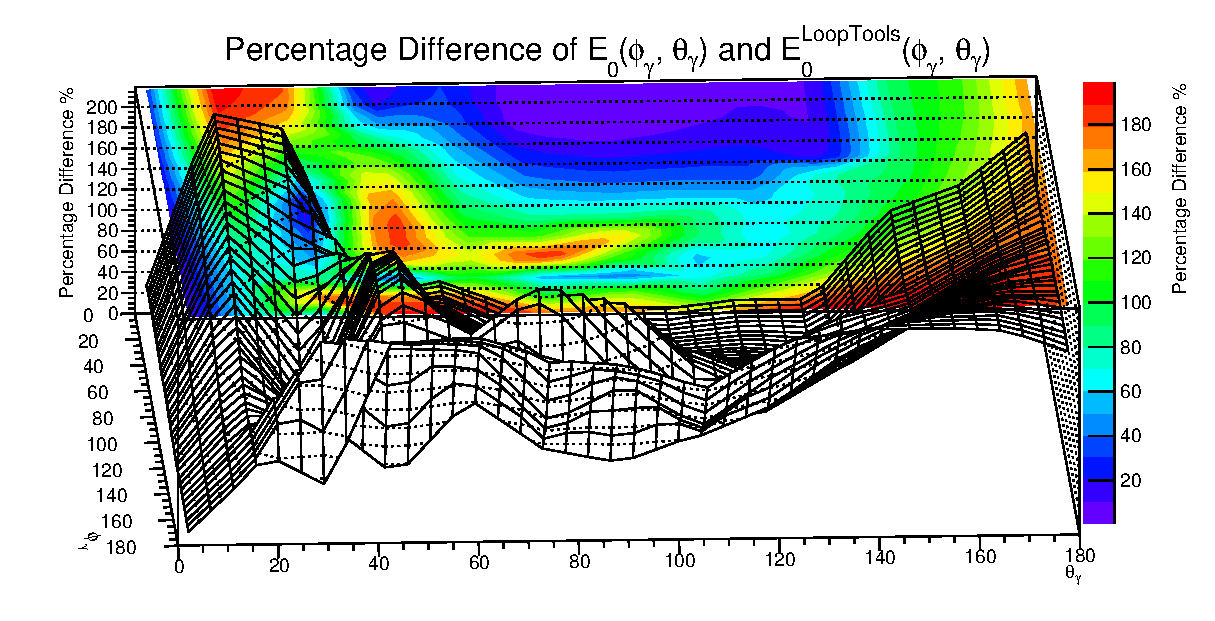
\includegraphics[scale=0.55]{30PD3.eps}\\
	\caption{ Percentage difference of $E_0(\phi_\gamma,\theta_\gamma)$ and $E_0^{LoopTools}(\phi_\gamma,\theta_\gamma)$ for $\sqrt{s}=500\text{ GeV}$, $M_{V_1}=91\text{ GeV}$, $M_{V_1}=91\text{ GeV}$ and $\theta'_1=30$ }
	\end{center}
\end{figure}

\begin{figure}
	\begin{center}
		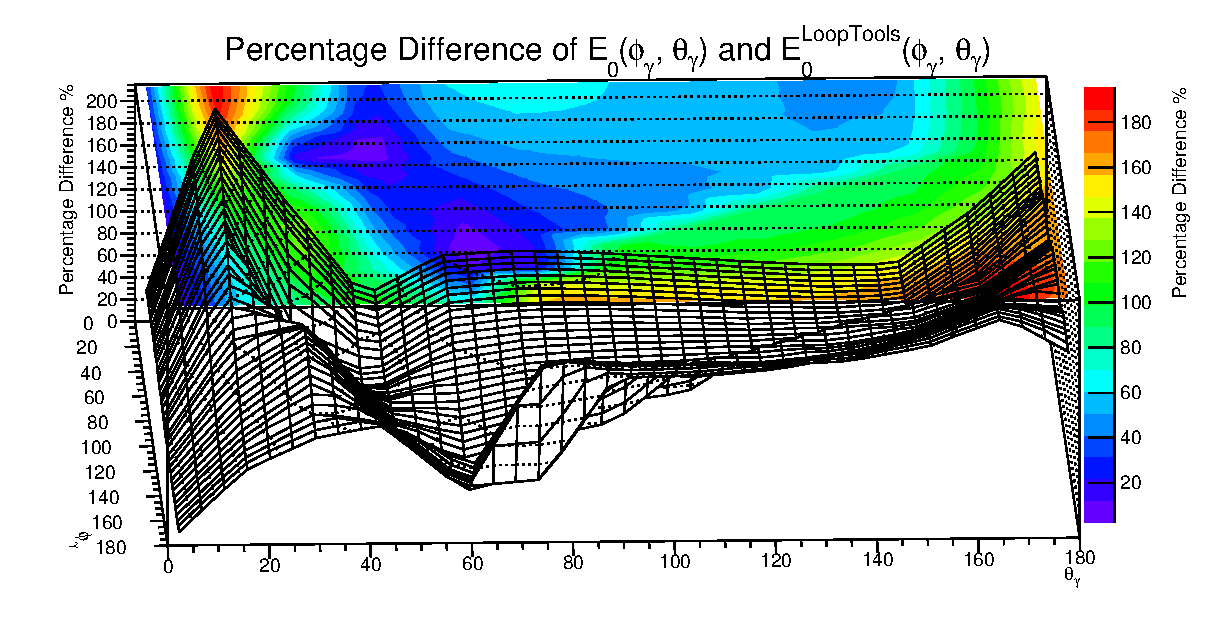
\includegraphics[scale=0.55]{45PD3.eps}\\
	\caption{ Percentage difference of $E_0(\phi_\gamma,\theta_\gamma)$ and $E_0^{LoopTools}(\phi_\gamma,\theta_\gamma)$ for $\sqrt{s}=500\text{ GeV}$, $M_{V_1}=91\text{ GeV}$, $M_{V_1}=91\text{ GeV}$ and $\theta'_1=45$ }
	\end{center}
\end{figure}

\begin{figure}
	\begin{center}
		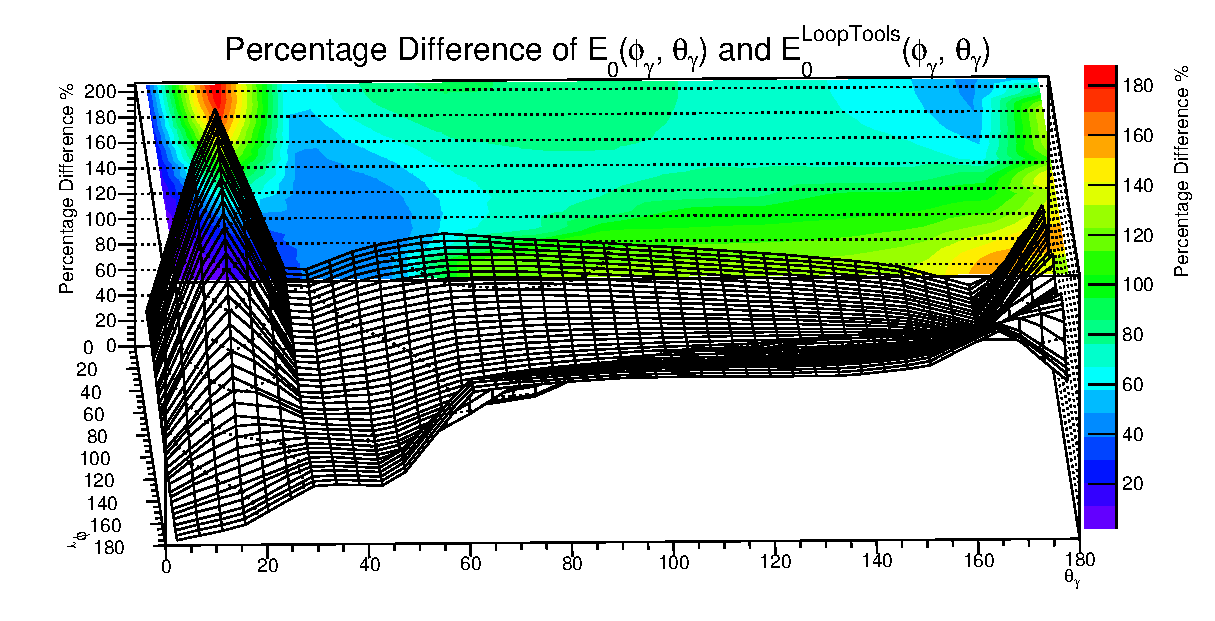
\includegraphics[scale=0.55]{60PD3.eps}\\
	\caption{ Percentage difference of $E_0(\phi_\gamma,\theta_\gamma)$ and $E_0^{LoopTools}(\phi_\gamma,\theta_\gamma)$ for $\sqrt{s}=500\text{ GeV}$, $M_{V_1}=91\text{ GeV}$, $M_{V_1}=91\text{ GeV}$ and $\theta'_1=60$ }
	\end{center}
\end{figure}

\begin{figure}
	\begin{center}
		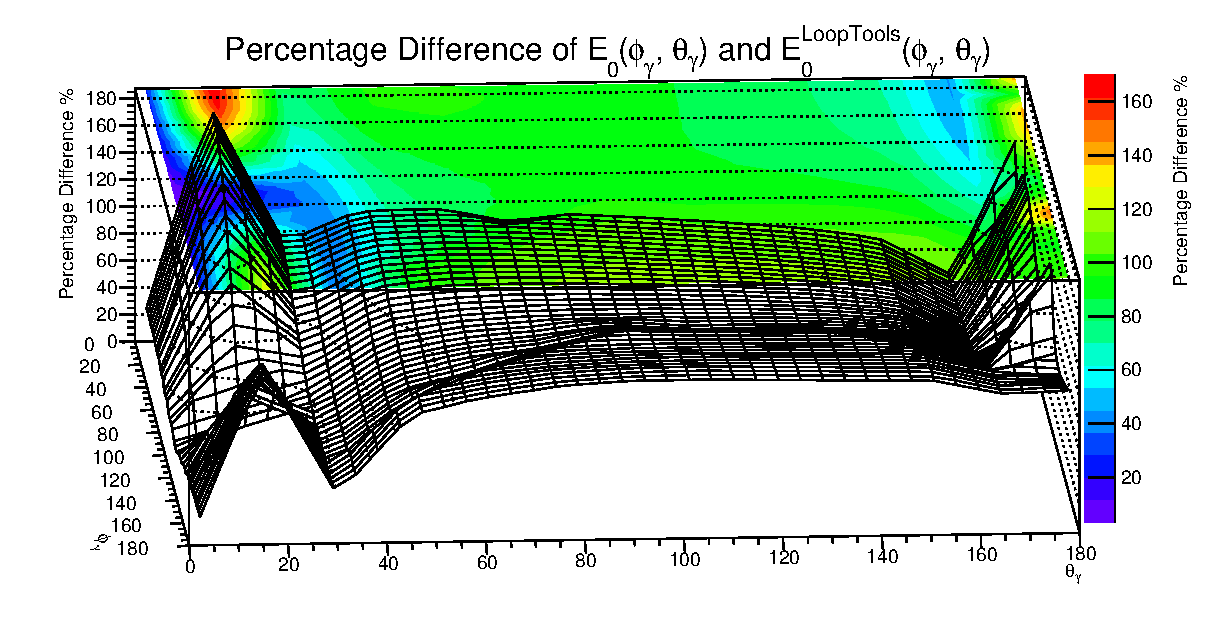
\includegraphics[scale=0.55]{75PD3.eps}\\
	\caption{ Percentage difference of $E_0(\phi_\gamma,\theta_\gamma)$ and $E_0^{LoopTools}(\phi_\gamma,\theta_\gamma)$ for $\sqrt{s}=500\text{ GeV}$, $M_{V_1}=91\text{ GeV}$, $M_{V_1}=91\text{ GeV}$ and $\theta'_1=75$ }
	\end{center}
\end{figure}

\begin{figure}
	\begin{center}
		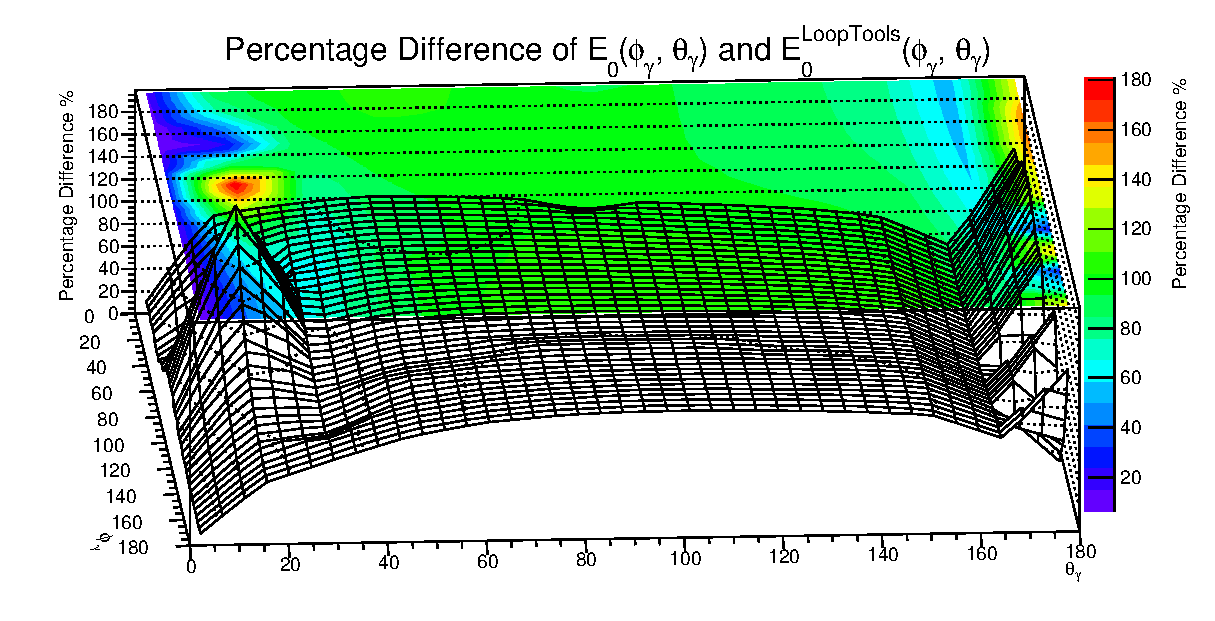
\includegraphics[scale=0.55]{90PD3.eps}\\
		\caption{ Percentage difference of $E_0(\phi_\gamma,\theta_\gamma)$ and $E_0^{LoopTools}(\phi_\gamma,\theta_\gamma)$ for $\sqrt{s}=500\text{ GeV}$, $M_{V_1}=91\text{ GeV}$, $M_{V_1}=91\text{ GeV}$ and $\theta'_1=90$ }
	\end{center}
\end{figure}

\begin{figure}
	\begin{center}
		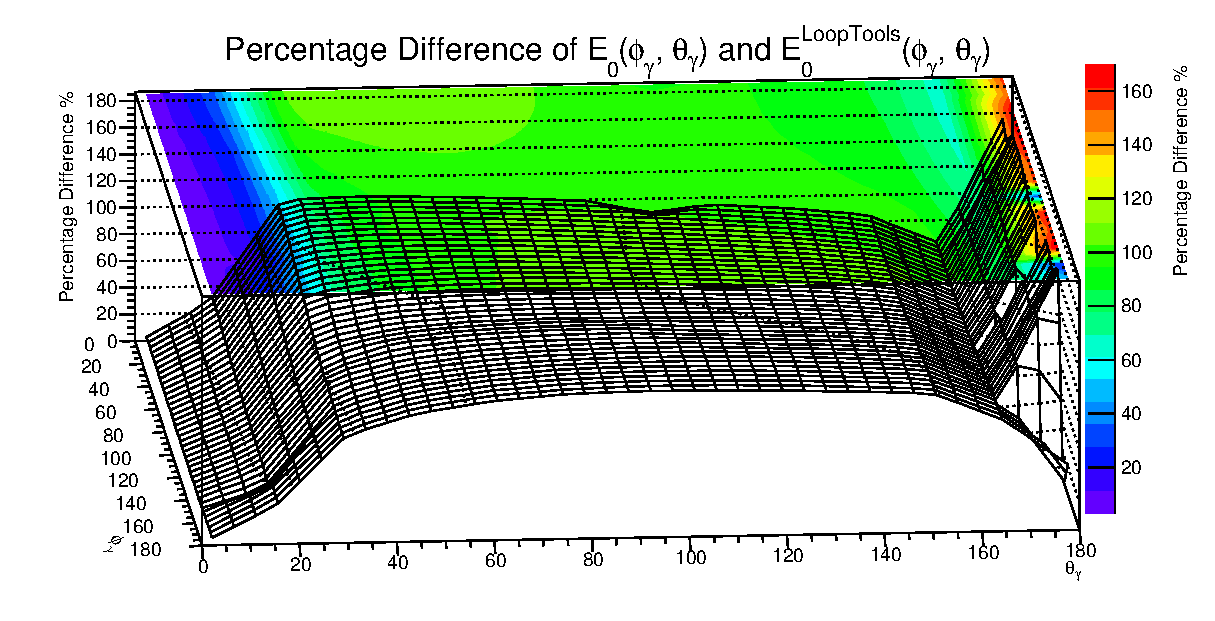
\includegraphics[scale=0.55]{105PD3.eps}\\
		\caption{ Percentage difference of $E_0(\phi_\gamma,\theta_\gamma)$ and $E_0^{LoopTools}(\phi_\gamma,\theta_\gamma)$ for $\sqrt{s}=500\text{ GeV}$, $M_{V_1}=91\text{ GeV}$, $M_{V_1}=91\text{ GeV}$ and $\theta'_1=105$ }
	\end{center}
\end{figure}

\begin{figure}
	\begin{center}
		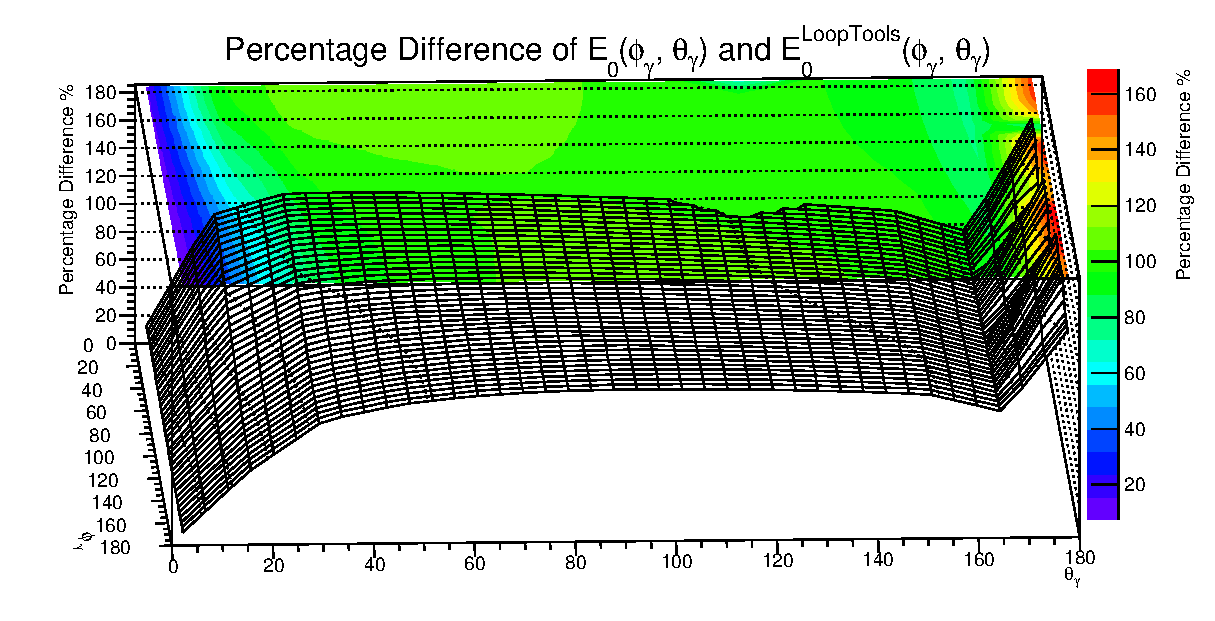
\includegraphics[scale=0.55]{120PD3.eps}\\
		\caption{ Percentage difference of $E_0(\phi_\gamma,\theta_\gamma)$ and $E_0^{LoopTools}(\phi_\gamma,\theta_\gamma)$ for $\sqrt{s}=500\text{ GeV}$, $M_{V_1}=91\text{ GeV}$, $M_{V_1}=91\text{ GeV}$ and $\theta'_1=120$ }
	\end{center}
\end{figure}


\begin{figure}
	\begin{center}
		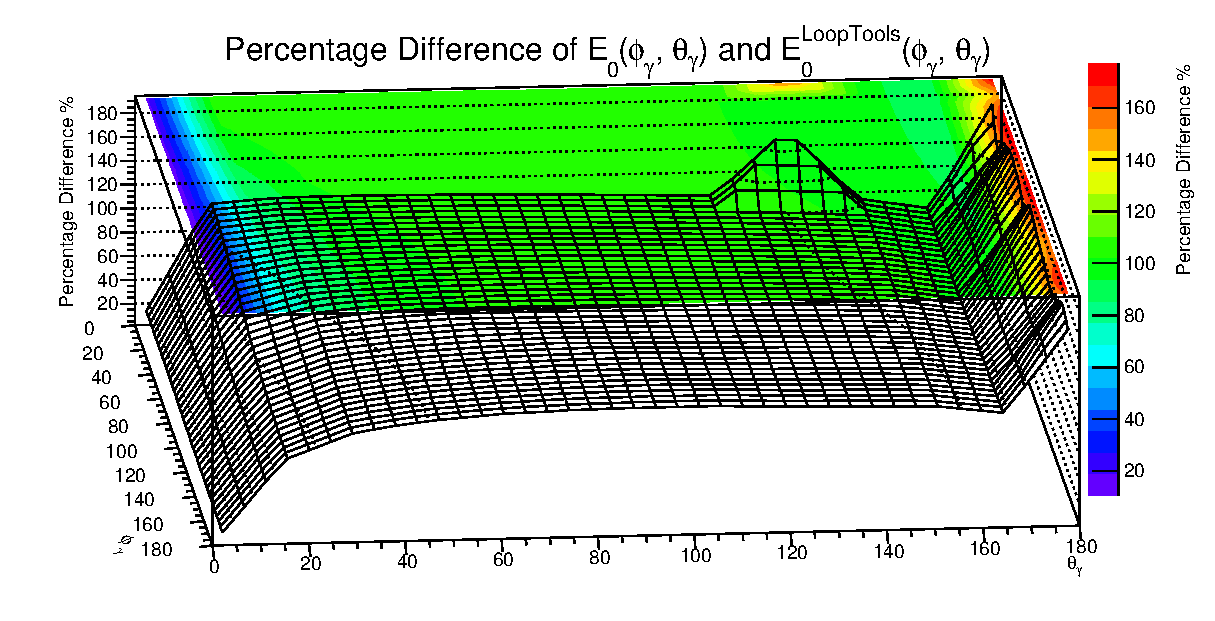
\includegraphics[scale=0.55]{135PD3.eps}\\
		\caption{ Percentage difference of $E_0(\phi_\gamma,\theta_\gamma)$ and $E_0^{LoopTools}(\phi_\gamma,\theta_\gamma)$ for $\sqrt{s}=500\text{ GeV}$, $M_{V_1}=91\text{ GeV}$, $M_{V_1}=91\text{ GeV}$ and $\theta'_1=135$ }
	\end{center}
\end{figure}


\begin{figure}
	\begin{center}
		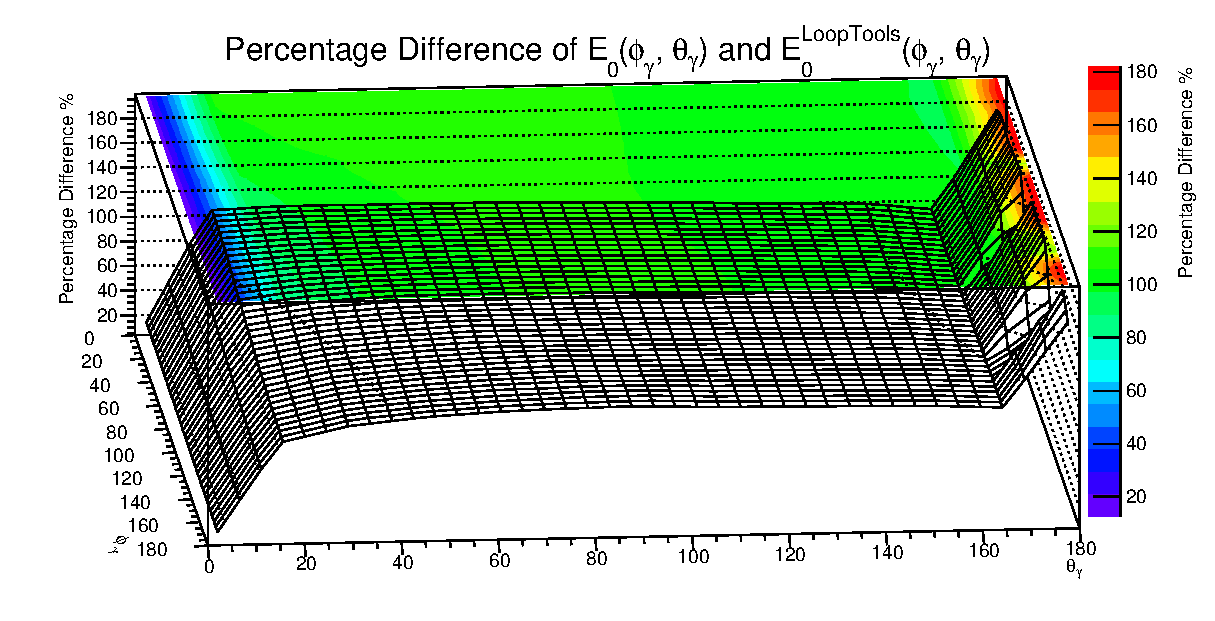
\includegraphics[scale=0.55]{150PD3.eps}\\
		\caption{ Percentage difference of $E_0(\phi_\gamma,\theta_\gamma)$ and $E_0^{LoopTools}(\phi_\gamma,\theta_\gamma)$ for $\sqrt{s}=500\text{ GeV}$, $M_{V_1}=91\text{ GeV}$, $M_{V_1}=91\text{ GeV}$ and $\theta'_1=150$ }
	\end{center}
\end{figure}

\begin{figure}
	\begin{center}
		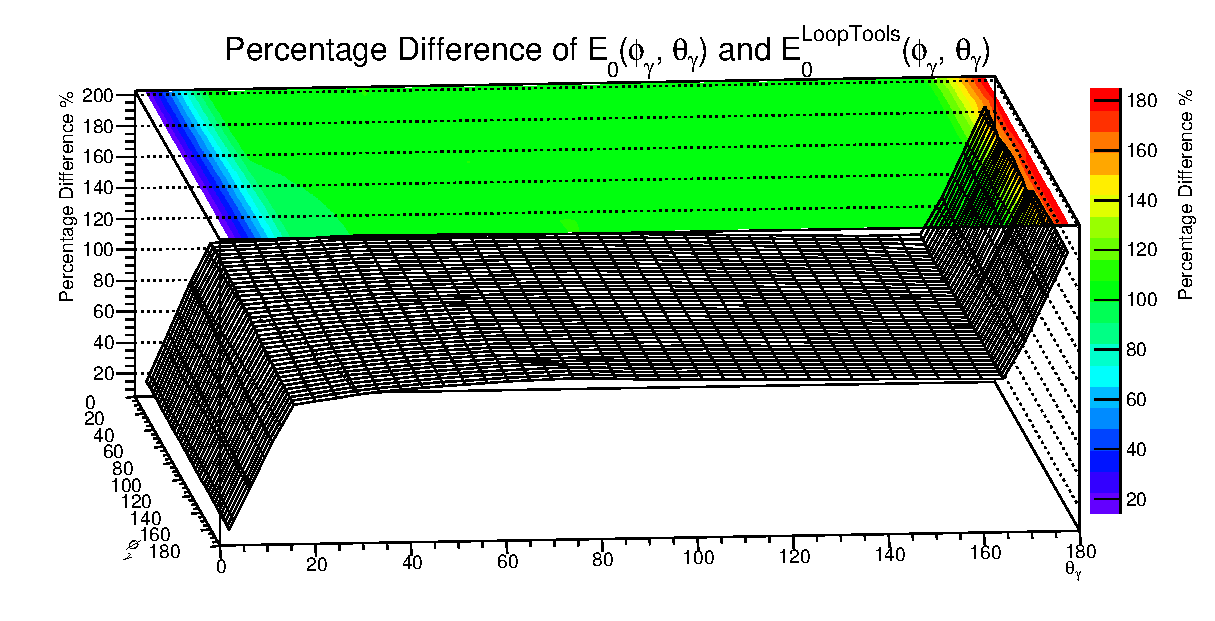
\includegraphics[scale=0.55]{165PD3.eps}\\
		\caption{ Percentage difference of $E_0(\phi_\gamma,\theta_\gamma)$ and $E_0^{LoopTools}(\phi_\gamma,\theta_\gamma)$ for $\sqrt{s}=500\text{ GeV}$, $M_{V_1}=91\text{ GeV}$, $M_{V_1}=91\text{ GeV}$ and $\theta'_1=165$ }
	\end{center}
\end{figure}


\begin{figure}
	\begin{center}
		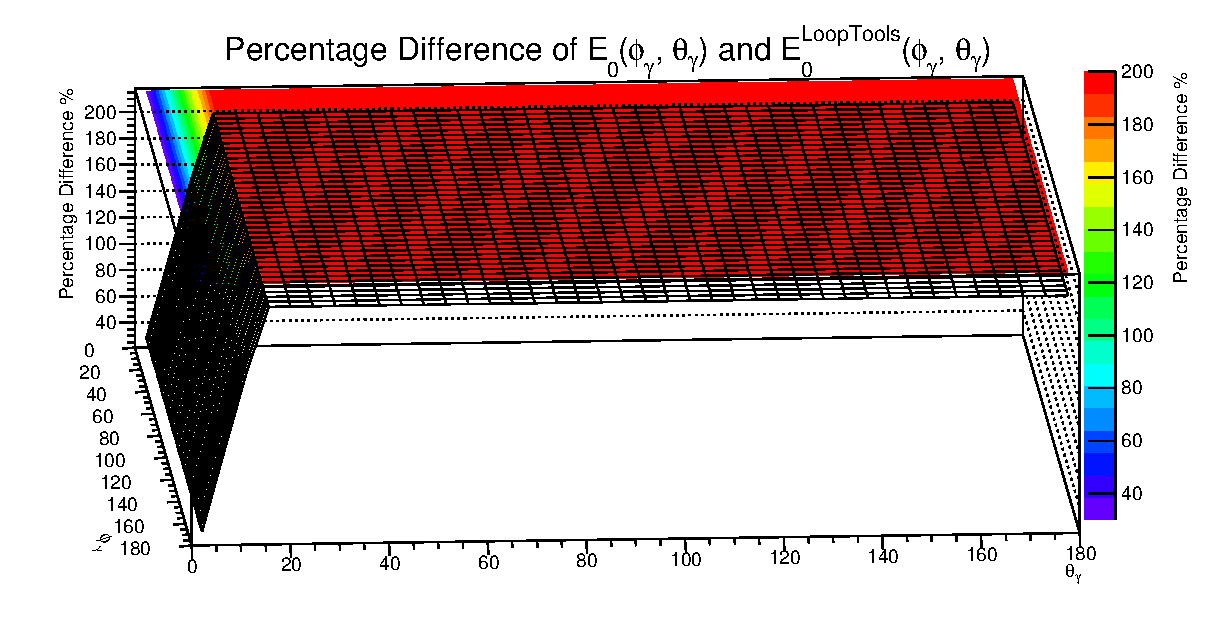
\includegraphics[scale=0.55]{180PD3.eps}\\
		\caption{ Percentage difference of $E_0(\phi_\gamma,\theta_\gamma)$ and $E_0^{LoopTools}(\phi_\gamma,\theta_\gamma)$ for $\sqrt{s}=500\text{ GeV}$, $M_{V_1}=91\text{ GeV}$, $M_{V_1}=91\text{ GeV}$ and $\theta'_1=180$ }
	\end{center}
\end{figure}

As we see, the result from magic spinor product method agrees with that from LoopTools in overall, except several regions. The percentage difference of $E_0(\phi_\gamma,\theta_\gamma)$ and $E_0^{\text{LoopTools}}(\phi_\gamma,\theta_\gamma)$ is insensitive with $\phi_\gamma$, but sensitive with $\theta'_1$. When $\theta'_1>90$, our result mainly fits to that from LoopTool in the region $(0<\phi_\gamma<180,\text{ }0<\theta_\gamma<20)$.
However, when $\theta'_1<75$, our result agrees greatly with that from Looptools.
